%!TEX root = ../dokumentation.tex

\chapter{Implementierung}

\section{BaklavaJS}

Eine der Anforderungen war es, das Modell visuell bearbeiten zu können. Dafür war es notwendig, einen Graph-Editor zu entwickeln. Ein solcher Editor erlaubt es, Knoten hinzuzufügen bzw. zu entfernen und sie miteinander zu verbinden.

Ein Knoten ist dabei wie eine mathematische Funktion: Er führt einen Algorithmus auf die Eingangsdaten aus und gibt die erzeugten Ausgangsdaten aus.

Visuell wird ein Knoten in BaklavaJS folgendermaßen dargestellt:

\begin{figure}[H]
    \centering
    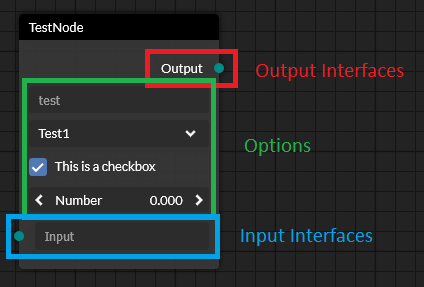
\includegraphics[width=.5\textwidth]{node_parts.png}
    \caption{Aufbau eines Knotens in BaklavaJS}
    \label{fig:nodeparts}
\end{figure}

Jeder Knoten besteht aus drei Teilen:
\begin{itemize}
    \item \textbf{Input Interfaces}: Die Eingangsschnittstellen eines Knotens werden benutzt, um Daten von anderen Knoten an diesen Knoten zu transferieren. Ist kein anderer Knoten verbunden, kann der Wert mittels eines Steuerelements auch direkt am Knoten eingestellt werden.
    \item \textbf{Options}: Hier können Werte eingestellt werden, die der Knoten für die Berechnung braucht, die aber beispielsweise zu komplex sind, um als Daten von anderen Knoten über Eingangsschnittstellen zu kommen.
    \item \textbf{Output Interfaces}: Die Ausgangsschnittstellen stellen das Ergebnis bereit, damit es von anderen Knoten benutzt werden kann.
\end{itemize}

\subsection{Ausführungsreihenfolge des Graphen}

\section{Random Sampling / Custom Random}